\section{Всякое по мелочам}

$ |a| = \left[ \begin{aligned}
	& a,\text{если\ } a\ge 0 \\
	& -a,\text{если\ } a < 0
\end{aligned}\right. $

\begin{center}
	Уравнение касательной к графику функции $\displaystyle y = f(x) $ в точке $\displaystyle M_0(x_0, f(x_0)) $ имеет вид:
	$ y = f'(x_0)\, x + (f(x_0) - f'(x_0)\, x_0) $
\end{center}

$ a^4 + a^2 + 1 = (a^2 - a + 1)\, (a^2 - a + 1) $

$ a^2 + b^2 = (a + b)^2 - 2\, a\, b $

$ (a \pm b)^3 = a^3\pm b^3\pm 3\, a\, b\, (a\pm b) $

$ \sqrt{\mathstrut a\pm \sqrt{\mathstrut b}} = \sqrt{\mathstrut \frac{a + \sqrt{\mathstrut a^2 - b}}{2}}\pm \sqrt{\mathstrut \frac{a - \sqrt{\mathstrut a^2 - b}}{2}} $

\begin{center}
	Квадратное уравнение:
	$ a\, x^2 + b\, x + c = 0 \Rightarrow $ $ \left[ \begin{aligned}
		& a\, (x - x_1)\, (x - x_2) = 0 \\
		& D = b^2 - 4\, a\, c \\
		& \left\{ \begin{aligned}
			& D > 0 \\
			& x_{1/2} = \frac{-b\pm \sqrt{\mathstrut D}}{2\, a}
		\end{aligned}\right. \\
		& \left\{ \begin{aligned}
			& D = 0 \\
			& x_{1/2} = \frac{-b}{2\, a}
		\end{aligned}\right.
	\end{aligned}\right. $
\end{center}

Симметричное уравнение:

$ 3x^4 + 4x^3 - x^2 + 4x + 3 = 0 $ - делим на $x^2$

$ 3\left(x^2 + \frac{1}{x^2}\right) + 4\left(x+\frac{1}{x}\right)-1 = 0 $

$ \left(x+\frac{1}{x}\right)^2 = \left(x^2+\frac{1}{x^2}\right) + 2 $

$ 3y^2 + 4y + 5 = 0 $

%--------------------------------------------------------------------------------%

\section{Свойства степени}

$ a^0 = 1 $

$ a^m = \underbrace{a\, a \, \ldots \, a }_{m сомножителей} $

$ a^{-m} = \frac{1}{a^m} $

$ a^n\, a^m = a^{n+m} $

$ \frac{a^n}{a^m} = a^{n-m} $

$ (a^n)^m = a^{n\, m} $

$ (a\, b)^n = a^n\, a^m $

$ \left(\frac{a}{b} \right)^n = \frac{a^n}{b^n} $

%--------------------------------------------------------------------------------%

\section{Свойства корня}

$ \sqrt[n]{\mathstrut a\, b} = \sqrt[n]{\mathstrut a} \, \sqrt[n]{\mathstrut b} $

$ \sqrt[n]{\mathstrut \frac{a}{b}} = \frac{\sqrt[n]{\mathstrut a}}{\sqrt[n]{\mathstrut b}} $

$ (\sqrt[n]{\mathstrut a})^k = \sqrt[n]{\mathstrut a^k} = a^{\frac{k}{n}} $

$ \sqrt[2n + 1]{\mathstrut -a} = -\sqrt[2n + 1]{\mathstrut a} $

$ \sqrt[n]{\mathstrut \sqrt[k]{\mathstrut a}} = \sqrt[n\, k]{\mathstrut a} $

$ \sqrt[n]{\mathstrut a} = \sqrt[n\, k]{\mathstrut a^k} $

$ \sqrt[2n]{\mathstrut a^{2n}} = |a| $

%--------------------------------------------------------------------------------%

\section{Свойства логарифма}

\begin{center}
	если $ a^x = b $, то $ \log_a b = x $.
\end{center}

$ a^{\log_b c} = c^{\log_b a} $

$ a^{\log_a x} = x $

$ \log_a (x\, y) = \log_a |x| + \log_a |y| $

$ \log_a \frac{x}{y} = \log_a |x| - \log_a |y| $

$ \log_a x^{2\, m} = 2m \log_a |x| $

$ \log_a b = \frac{\log_x b}{\log_x a} $

$ \log_a x = \frac{1}{\log_b a} $

$ \log_{a^k} x^m = \frac{m}{k} \log_a x $

$ \log_a 1 = 0 $

$ \log_a a = 1 $

$ \log_{\phi(x)} f(x) \ge \log_{\phi(x)} g(x) \Rightarrow $ $ \left[
	\begin{aligned}
		\left\{ \begin{aligned}
			& f(x) \ge g(x) \\
			& g(x) > 0 \\
			& \phi(x) > 1
		\end{aligned} \right.
		\left\{ \begin{aligned}
			& f(x) \le g(x) \\
			& f(x) > 0 \\
			& 0 < \phi(x) < 1
		\end{aligned} \right.
	\end{aligned} \right. $

$ \log_{\phi(x)} f(x) > \log_{\phi(x)} g(x) \Rightarrow $ $ \left[
	\begin{aligned}
		\left\{ \begin{aligned}
			& f(x) > g(x) \\
			& g(x) > 0 \\
			& \phi(x) > 1
		\end{aligned} \right.
		\left\{ \begin{aligned}
			& f(x) < g(x) \\
			& f(x) > 0 \\
			& 0 < \phi(x) < 1
		\end{aligned} \right.
	\end{aligned} \right. $

%--------------------------------------------------------------------------------%
	
\section{Комбинаторика}

$ P_n $ --- количество всех перестановок множества размером $ n $. Пример: все перестановки множества $abc$: $abc$, $acb$, $bac$, $bca$, $cab$, $cba$.

$ A^m_n $ --- количество размещений множества размером $ n $ по $ m $ элементов. Пример: все размещения множества $ \{1, 2, 3, 4, 5, 6 \} $ по два элемента: $ \{1, 2\} $, $ \{1, 3\} $, $ \{1, 4\} $, $ \{1, 5\} $, \dots, $ \{2, 1\} $, $ \{2, 3\} $,  \dots, $ \{5, 6\} $. При этом повторения вроде $ \{2, 2\} $ недопустимы. И размещения $ \{2, 1 \} $ и $ \{ 1, 2 \} $ считаются различными.

$ \widetilde{A}^m_n $ --- количество размещений множества размером $ n $ по $ m $ элементов с повторениями элементов в одном размещении. Т.е. повторения вроде $ \{2, 2\} $ допустимы.

$ C^m_n $ --- количество сочетаний множества размером $n$ по $m$ элементов. Сочетание --- размещение, в котором наборы вида $ \{2, 1 \} $ и $ \{ 1, 2 \} $ считаются одинаковыми.

$ \widetilde{C}^m_n $ --- количество сочетаний множества размером $n$ по $m$ элементов с повторениями. Т.е. повторения вроде $ \{2, 2\} $ допустимы.

$ A^m_n = \frac{n!}{(n-m)!} $

$ \widetilde{A}^m_n = n^m $

$ P_n = n! $

$ C^m_n = \frac{A^m_n}{P_m} = \frac{n!}{(n-m)!m!} $

$ C^m_n + C^{m+1}_n = C^{m+1}_{n+1} $

$ C^0_n + C^1_n + \dots + C^n_n = 2^n $

$ C^m_n = C^{n-m}_n $

$ \widetilde{C}^m_n = C^m_{n+m-1} = C^{n-1}_{n+m-1} = \frac{(n+m-1)!}{m!(n-1)!} $

$ T_{k+1} = C^k_n\cdot a^{n-k}b^k $

$ (a+b)^n = C^0_n\cdot a^n + C^1_n\cdot a^{n-1}b + \dots + C^n_n\cdot b^n $

%--------------------------------------------------------------------------------%
	
\section{Прогрессии}

\subsection{Арифметическая}

$ a_{n+1} = a_n + d $

$ a_n = a_1 + (n-1)\cdot d $

$ d = \frac{a_n-a_m}{n-m}, n \neq m $

$ a_n = \frac{a_{n+1} + a_{n-1}}{2} $

$ S_n = \frac{a_1 + a_n}{2}\cdot n $

$ S_n = \frac{2\cdot a_1 + (n-1)\cdot d}{2}\cdot n $

\subsection{Геометрическая}

$ b_n = b_{n-1}\cdot q $

$ b_n = b_1 \cdot q^{n-1} $

$ q^{n-m} = \frac{b_n}{b_m} $

$ b_n = \sqrt{b_{n+1}\cdot b_{n-1}}, b_n \neq 0 $

$ S_n = \frac{b_1 - b_n\cdot q}{1-q} $

$ S_n = \frac{b_1\cdot (1 - q^n}{1-q} $

$ S_\infty = \frac{b_1}{1-q}, \left|q\right| < 1 $

%--------------------------------------------------------------------------------%

\section{Тригонометрия}

\subsection{Графики}

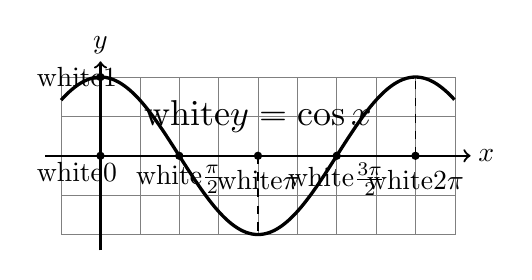
\begin{tikzpicture}

	% Grid
	\draw[step=0.5, very thin, gray] (-0.5,-1) grid ++(5, 2);

	% Graphs
	\draw[domain=-0.5:4.5,smooth,samples=500,variable=\x,black, very thick] plot ({\x},{cos(deg(\x/4*2*pi))});

	% Axes
	\draw[->, thick] (-0.7, 0) -- (4.7, 0);
	\draw[->, thick] (0, -1.2) -- (0, 1.2);

	\draw[-, dashed] (2, 0) -- (2, -1);
	\draw[-, dashed] (4, 0) -- (4, 1);

	% Nodes
	\draw (4.9,0) node {$x$};
	\draw (0, 1.4) node {$y$};

	\draw (-0.3, -0.2) node {\contour{white}{$0$}};
	\draw (-0.3, 1) node {\contour{white}{$1$}};

	\draw (1, -0.3) node {\contour{white}{$\frac{\pi}{2}$}};
	\draw (2, -0.3) node {\contour{white}{$\pi$}};
	\draw (3, -0.3) node {\contour{white}{$\frac{3\pi}{2}$}};
	\draw (4, -0.3) node {\contour{white}{$2\pi$}};

	\draw (2, 0.5) node[scale=1.3] {\contour{white}{$y=\cos x$}};

	% Points
	\fill [black] (0, 0) circle (1.5pt);
	\fill [black] (0, 1) circle (1.5pt);
	\fill [black] (1, 0) circle (1.5pt);
	\fill [black] (2, 0) circle (1.5pt);
	\fill [black] (3, 0) circle (1.5pt);
	\fill [black] (4, 0) circle (1.5pt);

\end{tikzpicture}
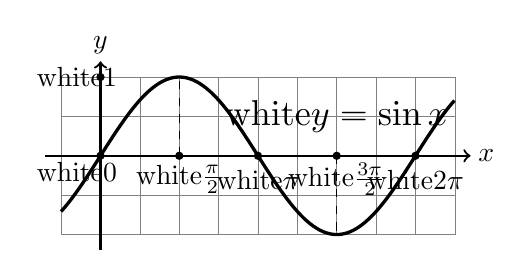
\begin{tikzpicture}

	% Grid
	\draw[step=0.5, very thin, gray] (-0.5,-1) grid ++(5, 2);

	% Graphs
	\draw[domain=-0.5:4.5,smooth,samples=500,variable=\x,black, very thick] plot ({\x},{sin(deg(\x/4*2*pi))});

	% Axes
	\draw[->, thick] (-0.7, 0) -- (4.7, 0);
	\draw[->, thick] (0, -1.2) -- (0, 1.2);

	\draw[-, dashed] (1, 0) -- (1, 1);
	\draw[-, dashed] (3, 0) -- (3, -1);

	% Nodes
	\draw (4.9,0) node {$x$};
	\draw (0, 1.4) node {$y$};

	\draw (-0.3, -0.2) node {\contour{white}{$0$}};
	\draw (-0.3, 1) node {\contour{white}{$1$}};

	\draw (1, -0.3) node {\contour{white}{$\frac{\pi}{2}$}};
	\draw (2, -0.3) node {\contour{white}{$\pi$}};
	\draw (3, -0.3) node {\contour{white}{$\frac{3\pi}{2}$}};
	\draw (4, -0.3) node {\contour{white}{$2\pi$}};

	\draw (3, 0.5) node[scale=1.3] {\contour{white}{$y=\sin x$}};

	% Points
	\fill [black] (0, 0) circle (1.5pt);
	\fill [black] (0, 1) circle (1.5pt);
	\fill [black] (1, 0) circle (1.5pt);
	\fill [black] (2, 0) circle (1.5pt);
	\fill [black] (3, 0) circle (1.5pt);
	\fill [black] (4, 0) circle (1.5pt);

\end{tikzpicture}

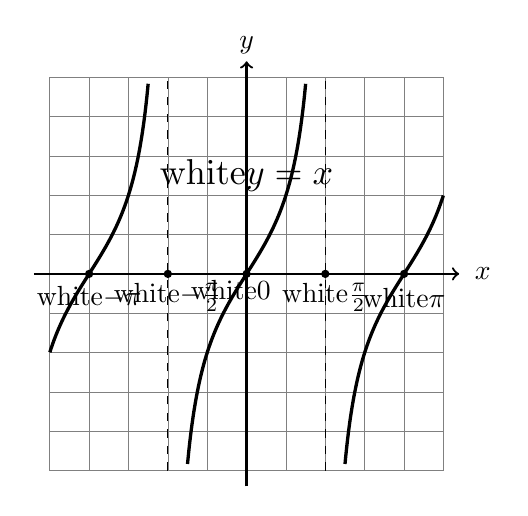
\begin{tikzpicture}

	% Grid
	\draw[step=0.5, very thin, gray] (-2.5,-2.5) grid ++(5, 5);

	% Graphs
	\draw[domain=-0.75:0.75	,smooth,samples=500,variable=\x,black, very thick] plot ({\x},{sin(deg(\x/4*2*pi))/cos(deg(\x/4*2*pi))});

	\draw[domain=1.25:2.5,smooth,samples=500,variable=\x,black, very thick] plot ({\x},{sin(deg(\x/4*2*pi))/cos(deg(\x/4*2*pi))});

	\draw[domain=-1.25:-2.5,smooth,samples=500,variable=\x,black, very thick] plot ({\x},{sin(deg(\x/4*2*pi))/cos(deg(\x/4*2*pi))});

	% Axes
	\draw[->, thick] (-2.7, 0) -- (2.7, 0);
	\draw[->, thick] (0, -2.7) -- (0, 2.7);

	\draw[-, dashed] (1, -2.5) -- (1, 2.5);
	\draw[-, dashed] (-1, -2.5) -- (-1, 2.5);

	% Nodes
	\draw (3,0) node {$x$};
	\draw (0, 2.9) node {$y$};

	\draw (-0.2, -0.2) node {\contour{white}{$0$}};

	\draw (1, -0.3) node {\contour{white}{$\frac{\pi}{2}$}};
	\draw (2, -0.3) node {\contour{white}{$\pi$}};
	\draw (-1, -0.3) node {\contour{white}{$-\frac{\pi}{2}$}};
	\draw (-2, -0.3) node {\contour{white}{$-\pi$}};

	\draw (0, 1.25) node[scale=1.3] {\contour{white}{$y=\tg x$}};

	% Points
	\fill [black] (0, 0) circle (1.5pt);
	\fill [black] (1, 0) circle (1.5pt);
	\fill [black] (2, 0) circle (1.5pt);
	\fill [black] (-1, 0) circle (1.5pt);
	\fill [black] (-2, 0) circle (1.5pt);

\end{tikzpicture}
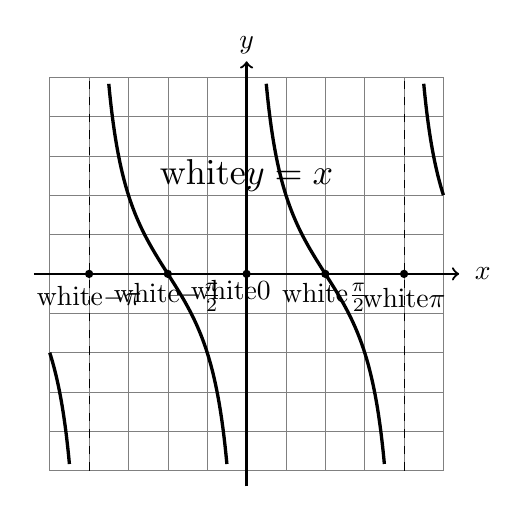
\begin{tikzpicture}

	% Grid
	\draw[step=0.5, very thin, gray] (-2.5,-2.5) grid ++(5, 5);

	% Graphs
	\draw[domain=0.25:1.75	,smooth,samples=500,variable=\x,black, very thick] plot ({\x},{cos(deg(\x/4*2*pi))/sin(deg(\x/4*2*pi))});

	\draw[domain=2.25:2.5,smooth,samples=500,variable=\x,black, very thick] plot ({\x},{cos(deg(\x/4*2*pi))/sin(deg(\x/4*2*pi))});

	\draw[domain=-0.25:-1.75,smooth,samples=500,variable=\x,black, very thick] plot ({\x},{cos(deg(\x/4*2*pi))/sin(deg(\x/4*2*pi))});

	\draw[domain=-2.25:-2.5,smooth,samples=500,variable=\x,black, very thick] plot ({\x},{cos(deg(\x/4*2*pi))/sin(deg(\x/4*2*pi))});

	% Axes
	\draw[->, thick] (-2.7, 0) -- (2.7, 0);
	\draw[->, thick] (0, -2.7) -- (0, 2.7);

	\draw[-, dashed] (2, -2.5) -- (2, 2.5);
	\draw[-, dashed] (-2, -2.5) -- (-2, 2.5);

	% Nodes
	\draw (3,0) node {$x$};
	\draw (0, 2.9) node {$y$};

	\draw (-0.2, -0.2) node {\contour{white}{$0$}};

	\draw (1, -0.3) node {\contour{white}{$\frac{\pi}{2}$}};
	\draw (2, -0.3) node {\contour{white}{$\pi$}};
	\draw (-1, -0.3) node {\contour{white}{$-\frac{\pi}{2}$}};
	\draw (-2, -0.3) node {\contour{white}{$-\pi$}};

	\draw (0, 1.25) node[scale=1.3] {\contour{white}{$y=\ctg x$}};

	% Points
	\fill [black] (0, 0) circle (1.5pt);
	\fill [black] (1, 0) circle (1.5pt);
	\fill [black] (2, 0) circle (1.5pt);
	\fill [black] (-1, 0) circle (1.5pt);
	\fill [black] (-2, 0) circle (1.5pt);

\end{tikzpicture}

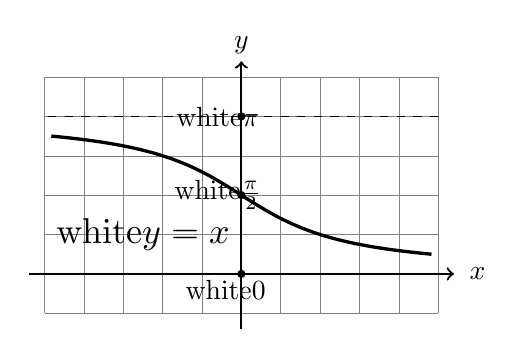
\begin{tikzpicture}

	% Grid
	\draw[step=0.5, very thin, gray] (-2.5,-0.5) grid ++(5, 3);

	% Graphs
	\draw[domain=0.25:1.75	,smooth,samples=500,variable=\x,black, very thick] plot ({cos(deg(\x/4*2*pi))/sin(deg(\x/4*2*pi))}, {\x});

	% Axes
	\draw[->, thick] (-2.7, 0) -- (2.7, 0);
	\draw[->, thick] (0, -0.7) -- (0, 2.7);

	\draw[-, dashed] (2.5, 2) -- (-2.5, 2);

	% Nodes
	\draw (3,0) node {$x$};
	\draw (0, 2.9) node {$y$};

	\draw (-0.2, -0.2) node {\contour{white}{$0$}};

	\draw (-0.3, 1) node {\contour{white}{$\frac{\pi}{2}$}};
	\draw (-0.3, 2) node {\contour{white}{$\pi$}};

	\draw (-1.25, 0.5) node[scale=1.3] {\contour{white}{$y=\arcctg x$}};

	% Points
	\fill [black] (0, 0) circle (1.5pt);
	\fill [black] (0, 1) circle (1.5pt);
	\fill [black] (0, 2) circle (1.5pt);

\end{tikzpicture}
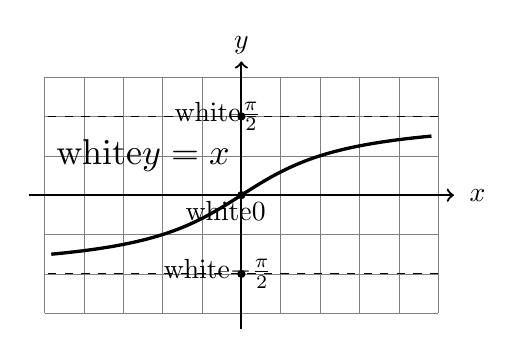
\begin{tikzpicture}

	% Grid
	\draw[step=0.5, very thin, gray] (-2.5,-1.5) grid ++(5, 3);

	% Graphs
	\draw[domain=-0.75:0.75	,smooth,samples=500,variable=\x,black, very thick] plot ({sin(deg(\x/4*2*pi))/cos(deg(\x/4*2*pi))}, {\x});

	% Axes
	\draw[->, thick] (-2.7, 0) -- (2.7, 0);
	\draw[->, thick] (0, -1.7) -- (0, 1.7);

	\draw[-, dashed] (2.5, 1) -- (-2.5, 1);
	\draw[-, dashed] (2.5, -1) -- (-2.5, -1);

	% Nodes
	\draw (3,0) node {$x$};
	\draw (0, 1.9) node {$y$};

	\draw (-0.2, -0.2) node {\contour{white}{$0$}};

	\draw (-0.3, 1) node {\contour{white}{$\frac{\pi}{2}$}};
	\draw (-0.3, -1) node {\contour{white}{$-\frac{\pi}{2}$}};

	\draw (-1.25, 0.5) node[scale=1.3] {\contour{white}{$y=\arctg x$}};

	% Points
	\fill [black] (0, 0) circle (1.5pt);
	\fill [black] (0, 1) circle (1.5pt);
	\fill [black] (0, -1) circle (1.5pt);

\end{tikzpicture}

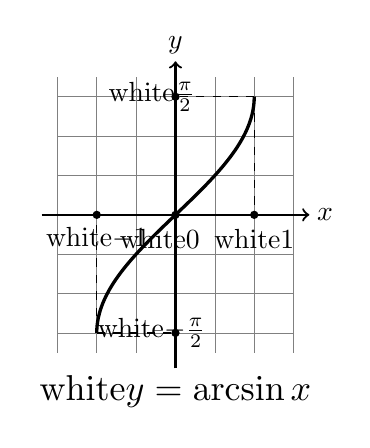
\begin{tikzpicture}

	% Grid
	\draw[step=0.5, very thin, gray] (-1.5,-1.75) grid ++(3, 3.5);

	% Graphs
	\draw[domain=-1.5:1.5, smooth,samples=500,variable=\x,black, very thick] plot ({sin(deg(\x/3*pi))}, {\x});

	% Axes
	\draw[->, thick] (-1.7, 0) -- (1.7, 0);
	\draw[->, thick] (0, -1.95) -- (0, 1.95);

	\draw[-, dashed] (-1, -1.5) -- (-1, 0);
	\draw[-, dashed] (1, 1.5) -- (1, 0);

	\draw[-, dashed] (-1, -1.5) -- (0, -1.5);
	\draw[-, dashed] (1, 1.5) -- (0, 1.5);

	% Nodes
	\draw (1.9,0) node {$x$};
	\draw (0, 2.15) node {$y$};

	\draw (-0.2, -0.3) node {\contour{white}{$0$}};

	\draw (-0.3, 1.5) node {\contour{white}{$\frac{\pi}{2}$}};
	\draw (-0.3, -1.5) node {\contour{white}{$-\frac{\pi}{2}$}};
	\draw (-1, -0.3) node {\contour{white}{$-1$}};
	\draw (1, -0.3) node {\contour{white}{$1$}};

	\draw (0, -2.25) node[scale=1.3] {\contour{white}{$y=\arcsin x$}};

	% Points
	\fill [black] (0, 0) circle (1.5pt);
	\fill [black] (0, 1.5) circle (1.5pt);
	\fill [black] (0, -1.5) circle (1.5pt);
	\fill [black] (1, 0) circle (1.5pt);
	\fill [black] (-1, 0) circle (1.5pt);

\end{tikzpicture}
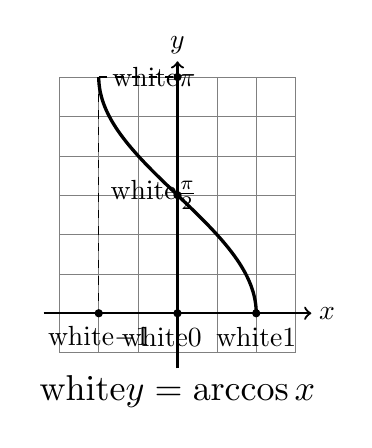
\begin{tikzpicture}

	% Grid
	\draw[step=0.5, very thin, gray] (-1.5,-0.5) grid ++(3, 3.5);

	% Graphs
	\draw[domain=0:3, smooth,samples=500,variable=\x,black, very thick] plot ({cos(deg(\x/3*pi))}, {\x});

	% Axes
	\draw[->, thick] (-1.7, 0) -- (1.7, 0);
	\draw[->, thick] (0, -0.7) -- (0, 3.2);

	\draw[-, dashed] (-1, 3) -- (-1, 0);
	\draw[-, dashed] (-1, 3) -- (0, 3);

	% Nodes
	\draw (1.9,0) node {$x$};
	\draw (0, 3.4) node {$y$};

	\draw (-0.2, -0.3) node {\contour{white}{$0$}};

	\draw (-0.3, 1.5) node {\contour{white}{$\frac{\pi}{2}$}};
	\draw (-0.3, 3) node {\contour{white}{$\pi$}};
	\draw (-1, -0.3) node {\contour{white}{$-1$}};
	\draw (1, -0.3) node {\contour{white}{$1$}};

	\draw (0, -1) node[scale=1.3] {\contour{white}{$y=\arccos x$}};

	% Points
	\fill [black] (0, 0) circle (1.5pt);
	\fill [black] (0, 1.5) circle (1.5pt);
	\fill [black] (0, 3) circle (1.5pt);
	\fill [black] (1, 0) circle (1.5pt);
	\fill [black] (-1, 0) circle (1.5pt);

\end{tikzpicture}

\subsection{Основное}

$ \sin^2 \alpha + \cos^2 \alpha = 1 $

$ \tg^2 \alpha + 1 = \frac{1}{\cos^2 \alpha} $

$ \ctg^2 \alpha + 1 = \frac{1}{\sin^2 \alpha} $

$ \tg \alpha\, \ctg \alpha = 1 $

$ \tg \alpha = \frac{\sin \alpha}{\cos \alpha} $

\subsection{Суммы углов}

$ \sin(\alpha\pm \beta) = \sin \alpha\, \cos \beta \pm \cos \alpha\, \sin \beta $

$ \cos(\alpha\pm \beta) = \cos \alpha\, \cos \beta \mp \sin \alpha\, \sin \beta $

$ \tg (\alpha \pm \beta) = \frac{\tg \alpha \pm \tg \beta}{1 \mp \tg \alpha \, \tg \beta} $

\subsection{Двойные и тройные углы}

$ \sin 2\, \alpha = 2\, \sin \alpha\, \cos \alpha $

$ \cos 2\, \alpha = \cos^2 \alpha - \sin^2 \alpha = $ $ 2\, \cos^2 \alpha - 1 = 1 - 2\, \sin^2 \alpha $

$ \tg 2\alpha = \frac{2\, \tg \alpha}{1 - \tg^2 \alpha} = \frac{2}{\ctg \alpha - \tg \alpha} $

$ \cos 3\, \alpha = 4\, \cos^3 \alpha - 3\, \cos \alpha $

$ \sin 3\, \alpha = 3\, \sin \alpha - 4\, \sin^3 \alpha $

$ \tg 3\, \alpha = \frac{3\, \tg \alpha - \tg^3 \alpha}{1 - 3\, \tg^2 \alpha} $

\subsection{Сумма функций}

$ \sin \alpha \pm \sin \beta = 2\, \sin \frac{\alpha \pm \beta}{2}\, \cos \frac{\alpha \mp \beta}{2} $

$ \cos \alpha \pm \cos \beta = 2\, \cos \frac{\alpha \pm \beta}{2}\, \cos \frac{\alpha \mp \beta}{2} $

$ a\, \sin \alpha + b\, \cos \alpha = \sqrt{\mathstrut a^2 + b^2}\, \sin \left(\alpha + \arcsin \frac{a}{\sqrt{\mathstrut a^2 + b^2}}\right) $

$ \tg \alpha \pm \tg \beta = \frac{\sin (\alpha \pm \beta)}{\cos \alpha\, \cos \beta} $

$ \ctg \alpha \pm \ctg \beta = \frac{\pm\sin (\alpha \pm \beta)}{\sin \alpha\, \sin \beta} $

$ \ctg \alpha \pm \tg \beta = \frac{\cos (\alpha \mp \beta)}{\sin \alpha\, \cos \beta} $

\subsection{Произведение функций}

$ \sin \alpha\, \cos \beta = \frac{1}{2}\, (\sin (\alpha - \beta) + \sin (\alpha + \beta)) $

$ \sin \alpha\, \sin \beta = \frac{1}{2}\, (\cos (\alpha - \beta) - \cos (\alpha + \beta)) $

$ \cos \alpha\, \cos \beta = \frac{1}{2}\, (\cos (\alpha - \beta) + \cos (\alpha + \beta)) $

\subsection{Понижение степени и половинный угол}

$ \cos^2 \alpha = \frac{1 + \cos 2\, \alpha}{2} $

$ \sin^2 \alpha = \frac{1 - \cos 2\, \alpha}{2} $

$ \sin^3 \alpha = \frac14(3\sin \alpha - \sin 3 \alpha) $

$ \cos^3 \alpha = \frac14(3\cos \alpha + \cos 3 \alpha) $

$ \tg \frac{\alpha}{2} = \pm \sqrt{\mathstrut \frac{1 - \cos \alpha}{1 + \cos \alpha}} = \frac{\sin \alpha}{1 + \cos \alpha} $

\subsection{Универсальная тригонометрическая подстановка}

\begin{tabu}[t]{||c|c||}
	\hline
		$ \tg \frac{\alpha}{2} = t $ & 		$ \sin \alpha = \frac{2t}{1 + t^2} $ \\
	\hline
		$ \alpha = 2\arctg t $ & 		$ \cos \alpha = \frac{1 - t^2}{1 + t^2} $ \\
	\hline
		$ d\alpha = \frac{2dt}{1+t^2}$ & 	$ \tg \alpha = \frac{2t}{1-t^2} $ \\
	\hline
\end{tabu}

\subsection{Таблица с суммой углов}

\begin{tabu}[t]{||c|c|c|c|c|c|c|c|c||}
	\hline
		$ \alpha $ &
			\specialcell{$ \frac{\pi}{2} - \alpha $ \\ $ 90^{\circ} - \alpha $} &
			\specialcell{$ \frac{\pi}{2} + \alpha $ \\ $ 90^{\circ} + \alpha $} &
			\specialcell{$ \pi - \alpha $ \\ $ 180^{\circ} - \alpha $} &
			\specialcell{$ \pi + \alpha $ \\ $ 180^{\circ} + \alpha $} &
			\specialcell{$ \frac{3\, \pi}{2} - \alpha $ \\ $ 270^{\circ} - \alpha $} &
			\specialcell{$ \frac{3\, \pi}{2} + \alpha $ \\ $ 270^{\circ} + \alpha $} &
			\specialcell{$ 2\, \pi - \alpha $ \\ $ 360^{\circ} - \alpha $} &
			\specialcell{$ 2\, \pi + \alpha $ \\ $ 360^{\circ} + \alpha $} \\
	\hline
		$ \sin \alpha $ & 	$ \cos \alpha $ & 	$ \cos \alpha $ & 	$ \sin \alpha $ & 	$ -\sin \alpha $ & 	$ -\cos \alpha $ & 	$ -\cos \alpha $ & 	$ -\sin \alpha $ & 	$ \sin \alpha $ \\
	\hline
		$ \cos \alpha $ & 	$ \sin \alpha $ & 	$ -\sin \alpha $ & 	$ -\cos \alpha $ & 	$ -\cos \alpha $ & 	$ -\sin \alpha $ & 	$ \sin \alpha $ & 	$ \cos \alpha $ & 	$ \cos \alpha $ \\
	\hline
		$ \tg \alpha $ & 	$ \ctg \alpha $ & 	$ -\ctg \alpha $ & 	$ -\tg \alpha $ & 	$ \tg \alpha $ & 	$ \ctg \alpha $ & 	$ -\ctg \alpha $ & 	$ -\tg \alpha $ & 	$ \tg \alpha $ \\
	\hline
		$ \ctg \alpha $ & 	$ \tg \alpha $ & 	$ -\tg \alpha $ & 	$ -\ctg \alpha $ & 	$ \ctg \alpha $ & 	$ \tg \alpha $ & 	$ -\tg \alpha $ & 	$ -\ctg \alpha $ & 	$ \ctg \alpha $ \\
	\hline
\end{tabu}

\subsection{Тригонометрические уравнения}

\begin{tabu}[t]{||c|c|c||}
	\hline
		Уравнение & Решение & Условие \\
	\hline
		$ \sin x = a $ & 	$ x = (-1)^k\, \arcsin a + \pi\, k $ & 	$ |a| \le 1 $ \\
	\hline
		$ \cos x = a $ & 	$ x = \pm \arccos a + 2\, \pi\, k $ & 	$ |a| \le 1 $ \\
	\hline
		$ \tg x = a $ & 	$ x = \arctg a + \pi\, k $ & 	$ - $ \\
	\hline
		$ \ctg x = a $ & 	$ x = \arcctg a + \pi\, k $ & 	$ - $ \\
	\hline
\end{tabu}

Частные случаи:

\begin{tabu}[t]{||c|c||c|c||}
	\hline
		Уравнение & Решение & Уравнение & Решение \\
	\hline
		$ \sin x = 0 $ & 	$ x = \pi\, k $ & 				$ \cos x = 0 $ &	$ x = \frac{\pi}{2} + \pi\, k $ \\
	\hline
		$ \sin x = 1 $ & 	$ x = \frac{\pi}{2} + 2\, \pi\, k $ & 	$ \cos x = 1 $ & 	$ x = 2\, \pi\, k $ \\
	\hline
		$ \sin x = -1 $ & 	$ x = -\frac{\pi}{2} + 2\, \pi\, k $ & 	$ \cos x = -1 $ & 	$ x = \pi + 2\, \pi\, k $ \\
	\hline
		$ \tg x = 0 $ & 	$ x = \pi\, k $ & 				$ \ctg x = 0 $ & 	$ x = \frac{\pi}{2} + \pi\, k $ \\
	\hline
		$ \tg x = 1 $ & 	$ x = \frac{\pi}{4} + \pi\, k $ & 		$ \ctg x = 1 $ & 	$ x = \frac{\pi}{4} + \pi\, k $ \\
	\hline
		$ \tg x = -1 $ & 	$ x = -\frac{\pi}{4} + \pi\, k $ & 		$ \ctg x = -1 $ & 	$ x = \frac{3\, \pi}{4} + \pi\, k $ \\
	\hline
\end{tabu}

\subsection{Обратные тригонометрические функции:}

\begin{tabu}[t]{||c||c||c||}
	\hline
		$ \sin\arcsin x = x $            & $ \sin\arccos x = \sqrt{1-x^2} $          & $ \arcsin(-x) = -\arcsin x $              \\
	\hline
		$ \arcsin\sin\alpha = \alpha $   & $ \cos\arcsin x = \sqrt{1-x^2} $            & $ \arccos(-x) = \pi - \arccos x $         \\
	\hline
	\hline
		$ \cos\arccos x = x $            & $ \sin\arctg x = \frac{x}{\sqrt{1+x^2}} $ & $ \arctg(-x) = -\arctg x $                \\
	\hline
		$ \arccos\cos\alpha = \alpha $   & $ \cos\arctg x = \frac{1}{\sqrt{1+x^2}} $ & $ \arcctg(-x) = \pi - \arcctg x $         \\
	\hline
	\hline
		$ \tg\arctg x = x $              & $ \tg\arcsin x = \frac{x}{\sqrt{1-x^2}} $ & $ \arcsin x + \arccos x = \frac{\pi}{2} $ \\
	\hline
		$ \arctg\tg\alpha = \alpha $     & $ \tg\arccos x = \frac{\sqrt{1-x^2}}{x} $ & $ \arctg x + \arcctg x = \frac{\pi}{2} $  \\
	\hline
\end{tabu}

\subsection{Сумма обратных тригонометрических функций}

\begin{tabu}[t]{||c||}
	\hline
		$ \arcsin x - \arcsin y =  \arcsin x + \arcsin(-y) $ \\
		$ \Sigma_{\sin{}} = \arcsin\left(x\sqrt{\mathstrut 1-y^2}+y\sqrt{\mathstrut 1-x^2}\right) $ \\
	\hline
		$ \boxed{\arcsin x + \arcsin y =} $ \\
		$ \left\{ \begin{aligned}
			\Sigma_{\sin{}}, \quad & xy \leqslant 0,\quad & x^2 + y^2 \leqslant 1 \\
			\pi-\Sigma_{\sin{}}, \quad & x > 0, y > 0,\quad  & x^2 + y^2 > 1 \\
			-\pi-\Sigma_{\sin{}}, \quad & x < 0, y < 0,\quad & x^2 + y^2 > 1 \\
		\end{aligned} \right. $ \\
	\hline
	\hline
		$ \arccos x - \arccos y =  -\pi + \arccos x + \arccos(-y) $ \\
		$ \Sigma_{\cos{}} = \arccos\left(xy+\sqrt{\mathstrut 1-x^2}\sqrt{\mathstrut 1-y^2}\right) $ \\
	\hline
		$ \boxed{\arccos x + \arccos y =} $
		$ \left\{ \begin{aligned}
			\Sigma_{\cos{}}, \quad & x \geqslant -y \\
			2\pi-\Sigma_{\cos{}}, \quad & x < -y
		\end{aligned} \right. $ \\
	\hline
	\hline
		$ \arctg x - \arctg y =  \arctg x + \arctg(-y) $ \\
		$ \Sigma_{\tg{}} = \arctg\frac{x+y}{1-xy} $ \\
	\hline
		$ \boxed{\arctg x + \arctg y =} $
		$ \left\{ \begin{aligned}
			\Sigma_{\tg{}}, \quad & & xy < 1 \\
			\pi+\Sigma_{\tg{}}, \quad & x > 0, \quad & xy>1 \\
			-\pi+\Sigma_{\tg{}}, \quad & x < 0, \quad & xy>1 \\
		\end{aligned} \right. $ \\
	\hline
\end{tabu}

\subsection{Таблица значений функций}

\subsubsection{Для стандартных углов}

\begin{tabu}[t]{||c|c|c|c|c|c|c|c|c|c||}
	\hline
		$ \alpha $ &
		$ 0 $ &
		$ \cfrac{\pi}{6} $ &
		$ \cfrac{\pi}{4} $ &
		$ \cfrac{\pi}{3} $ &
		$ \cfrac{\pi}{2} $ &
		$ \cfrac{2\pi}{3} $ &
		$ \cfrac{3\pi}{4} $ &
		$ \cfrac{5\pi}{6} $ &
		$ \pi $ \\
	\hline
		$ \alpha^{\circ} $ &
		$ 0^{\circ} $ &
		$ 30^{\circ} $ &
		$ 45^{\circ} $ &
		$ 60^{\circ} $ &
		$ 90^{\circ} $ &
		$ 120^{\circ} $ &
		$ 135^{\circ} $ &
		$ 150^{\circ} $ & 
		$ 180^{\circ} $ \\
	\hline
		$ \sin \alpha $ & 	$ 0 $ & 	$ \cfrac{1}{2} $ & 	$ \cfrac{\sqrt{2}}{2} $ & 	$ \cfrac{\sqrt{3}}{2} $ & 	$ 1 $ & 	$ \cfrac{\sqrt{3}}{2} $ & 	$ \cfrac{\sqrt{2}}{2} $ & 	$ \cfrac{1}{2} $ & $ 0 $ \\
	\hline
		$ \cos \alpha $ & 	$ 1 $ & 	$ \cfrac{\sqrt{3}}{2} $ & 	$ \cfrac{\sqrt{2}}{2} $ & 	$ \cfrac{1}{2} $ & 	$ 0 $ & 	$ -\cfrac{1}{2} $ & 	$ -\cfrac{\sqrt{2}}{2} $ & 	$ -\cfrac{\sqrt{3}}{2} $ & $ -1 $ \\
	\hline
		$ \tg \alpha $ & 	$ 0 $ & 	$ \cfrac{\sqrt{3}}{3} $ & 	$ 1 $ & 	$ \sqrt{3} $ & 	--- & 	$ -\sqrt{3} $ & 	$ -1 $ & 	$ -\cfrac{\sqrt{3}}{3} $ & $ 0 $ \\
	\hline
		$ \ctg \alpha $ & 	--- & 	$ \sqrt{3} $ & 	$ 1 $ & 	$ \cfrac{\sqrt{3}}{3} $ & 	0 & 	$ -\cfrac{\sqrt{3}}{3} $ & 	$ -1 $ & 	$ -\sqrt{3} $ & --- \\
	\hline
\end{tabu}

\subsubsection{Для особых углов}

\begin{tabu}[t]{||c|c|c|c|c|c|c||}
	\hline
		$ \alpha $ &
			$ \cfrac{\pi}{12}  =  15^{\circ} $ &
			$ \cfrac{\pi}{10} = 18^{\circ} $ &
			$ \cfrac{\pi}{5} = 36^{\circ} $ &
			$ \cfrac{3\pi}{10} = 54^{\circ} $ &
			$ \cfrac{2\pi}{5} = 72^{\circ} $ &
			$ \cfrac{5\pi}{12} = 75^{\circ} $ \\
	\hline
		$ \sin \alpha $ &
		$ \cfrac{\sqrt{3}-1}{2\sqrt{2}} $ & 	
		$ \cfrac{\sqrt{5}-1}{4} $ & 	
		$ \cfrac{\sqrt{5-\sqrt{5}}}{2\sqrt{2}} $ & 	
		$ \cfrac{\sqrt{5}+1}{4} $ & 	
		$ \cfrac{\sqrt{5+\sqrt{5}}}{2\sqrt{2}} $ & 	
		$ \cfrac{\sqrt{3}+1}{2\sqrt{2}} $ \\
	\hline
		$ \cos \alpha $ & 	
		$ \cfrac{\sqrt{3}+1}{2\sqrt{2}} $ & 	
		$ \cfrac{\sqrt{5+\sqrt{5}}}{2\sqrt{2}} $ & 	
		$ \cfrac{\sqrt{5}+1}{4} $ & 	
		$ \cfrac{\sqrt{5-\sqrt{5}}}{2\sqrt{2}} $ & 	
		$ \cfrac{\sqrt{5}-1}{4} $ & 	
		$ \cfrac{\sqrt{3}-1}{2\sqrt{2}} $ \\
	\hline
		$ \tg \alpha $ & 	
		$ 2-\sqrt{3} $ & 	
		$ \sqrt{1-\cfrac{2}{\sqrt{5}}} $ & 	
		$ \sqrt{5-2\sqrt{5}} $ & 	
		$ \sqrt{1+\cfrac{2}{\sqrt{5}}} $ & 	
		$ \sqrt{5+2\sqrt{5}} $ & 	
		$ 2+\sqrt{3} $ \\
	\hline
		$ \ctg \alpha $ & 
		$ 2+\sqrt{3} $ & 	
		$ \sqrt{5+2\sqrt{5}} $ & 	
		$ \sqrt{1+\cfrac{2}{\sqrt{5}}} $ & 	
		$ \sqrt{5-2\sqrt{5}} $ & 	
		$ \sqrt{1-\cfrac{2}{\sqrt{5}}} $ & 	
		$ 2-\sqrt{3} $ \\
	\hline
\end{tabu}

\subsubsection{Для нестандартных углов}

%--------------------------------------------------------------------------------%

\section{Гиперболические функции}

\subsection{Графики}

\subsection{Основные}

$ \ch^2 x - \sh^2 x = 1 $

$ \ctg^2 x - 1 = \frac{1}{\sh^2 x} $

$ 1 - \th^2 x = \frac{1}{\ch^2 x} $

$ \th x \, \cth x = 1 $

$ \th x = \frac{\sh x}{\ch x} $

\subsection{Суммы углов}

$ \sh(x \pm y) = \sh x \, \ch y \pm \sh y \, \ch x $

$ \ch(x \pm y) = \ch x \, \ch y \pm \sh y \, \sh x $

$ \th(x \pm y) = \frac{\th x \pm \th y}{1 \pm \th x \, \th y} $

\subsection{Двойные и тройные углы}

$ \sh 2x = 2\sh x \, \ch x $

$ \ch 2x = \ch^2 x + \sh^2 x = 2\ch^2 x - 1 = 1 + 2\sh^2 x $

$ \th 2x = \frac{2\th x}{1 + \th^2 x} = \frac{2}{\th x + \cth x} $

$ \sh 3x = 4\sh^3 x + 3\sh x $

$ \ch 3x = 4\ch^3 x - 3\ch x $

$ \th 3x = \th x \cdot \frac{3+\th^2 x}{1 + 3\th^2 x} $

\subsection{Сумма функций}

$ \sh x \pm \sh y = 2\sh\frac{x\pm y}{2}\,\ch\frac{x\mp y}{2} $

$ \ch x + \ch y = 2\ch\frac{x+y}{2}\,\ch\frac{x-y}{2} $

$ \ch x - \ch y = 2\sh\frac{x+ y}{2}\,\sh\frac{x- y}{2} $

$ \th x \pm \th y = 2\frac{\sh(x\pm y)}{\ch x\, \ch y} $

\subsection{Произведение функций}

$ \sh x \, \sh y = \frac12(\ch(x+y)-\ch(x-y)) $

$ \sh x \, \ch y = \frac12(\sh(x+y)+\sh(x-y)) $

$ \ch x \, \ch y = \frac12(\ch(x+y)+\ch(x-y)) $

\subsection{Понижение степени и половинный угол}

$ \ch^2 x = \frac{\ch 2x+1}{2} $

$ \th^2 x = \frac{\ch 2x-1}{2} $ 

\subsection{Универсальная гиперболическая подстановка}



\subsection{Обратные гиперболические функции}

\subsection{Сумма обратных гиперболических функций}

%--------------------------------------------------------------------------------%

\section{Математический анализ}

\subsection{Пределы}

\subsection{Ряды}

\subsection{Дифференциирование}

\subsubsection{Свойства}

$ (f(x) + g(x))' = f'(x) + g'(x) $

$ (f(x)\cdot g(x))' = f'(x)\cdot g(x) + f(x)\cdot g'(x) $

$ (k\cdot f(x))' = k\cdot f'(x), k \in R $

$ \left(\frac{f(x)}{g(x)}\right)' = \frac{f'(x)\cdot g(x) - f(x)\cdot g'(x)}{g^2(x)} $

$ (h(f(x)))' = h'(f(x)) \cdot f'(x) $

\subsubsection{Таблица производных}

\begin{tabu}[t]{||c|c||c|c||}
	\hline
		$ f(x) $ & $ f'(x) $ & $ f(x) $ &  $ f'(x) $ \\
	\hline
		$ c $ & $ 0 $ & $ \tg x $ &  $ \frac{1}{\cos^2 x} $ \\
	\hline
		$ x^n $ & $ nx^{n-1} $ & $ \ctg x $ &  $ -\frac{1}{\sin^2 x} $ \\
	\hline
		$ \sqrt{x} $ & $ \frac{1}{2\sqrt{x}} $ & $ \arcsin x $ &  $ \frac{1}{\sqrt{1-x^2}} $ \\
	\hline
		$ \frac{1}{x} $ & $ -\frac{1}{x^2} $ & $ \arccos x $ &  $ -\frac{1}{\sqrt{1-x^2}} $ \\
	\hline
		$ a^x $ & $ a^x \ln a $ & $ \arctg x $ &  $ \frac{1}{1+x^2} $ \\
	\hline
		$ e^x $ & $ e^x $ & $ \arcctg x $ &  $ -\frac{1}{1+x^2} $ \\
	\hline
		$ \log_a x $ & $ \frac{1}{x \ln a} $ & $ \sqrt[n]{x} $ &  $ \frac{1}{n\sqrt[n]{x^n-1}} $ \\
	\hline
		$ \ln x $ & $ \frac{1}{x} $ & $ \frac{1}{x^n} $ &  $ -\frac{n}{x^{n+1}} $ \\
	\hline
		$ \sin x $ & $ \cos x $ & $ \frac{1}{\sqrt{x}} $ &  $ -\frac{1}{2x\sqrt{x}} $ \\
	\hline
		$ \cos x $ & $ -\sin x $ & $ - $ &  $ - $ \\
	\hline
\end{tabu}

\subsection{Интегрирование}

\subsubsection{Свойства}

$ \int (f(x) \pm g(x)) dx = \int f(x) dx \pm \int g(x) dx $

$ \int k\cdot f(x) dx = k\cdot \int f(x) dx, k \in \mathbb{R} $

$ \int\limits_a^b f(x) dx = \left.F(x)\right|_b^a = F(b) - F(a) $

\subsubsection{Таблица неопределенных интегралов}

Константа интегрирования будет опускаться для уменьшения размеров.

$ \int x^a dx = \frac{x^{a+1}}{a+1}, a \neq -1 $

$ \int \frac{1}{x} dx = \ln|x| $

$ \int \sin x dx = -\cos x $

$ \int \cos x dx = \sin x $

$ \int \frac{1}{\cos^2 x} dx = \tg x $

$ \int \frac{1}{\sin^2 x} = -\ctg x $

$ \int a^x dx = \frac{a^x}{\ln a}, a>0, a \neq 1 $

$ \int e^x dx = e^x $

$ \int \frac{1}{x^2 + a^2} dx = \frac{1}{a} \arctg\frac{x}{a} $

$ \int \frac{1}{x^2 - a^2} dx = \frac{1}{2a} \ln\left|\frac{x-a}{x+a}\right|, a \neq 0, |x| \neq |a| $

$ \int \frac{1}{\sqrt{a^2-x^2}} dx = \arcsin\frac{x}{a} $

$ \int \frac{1}{\sqrt{x^2\pm a^2}} dx = \ln\left|x+\sqrt{x^2\pm a^2}\right|, x^2-a^2 > 0 $

$ \int \frac{1}{\sin x} dx = \ln\left|\tg\frac{x}{2}\right| $

$ \int \frac{1}{\cos x} dx = \ln\left|\tg\left(\frac{x}{2} + \frac{\pi}{2}\right)\right| $

$ \int \tg x dx = -\ln|\cos x| $

$ \int \ctg x dx = \ln|\sin x| $

$ \int \ln x dx = x(\ln x -1) $

\subsubsection{Приложения определенного интеграла}

Площадь под графиком:

$ S_{(a; b)}(f) = \int\limits_a^b f(x) dx $

$ S_{(t_1; t_2)}(x, y) = \int\limits_{t_1}^{t_2} y(t)\cdot x'(t) dt $ 

$ S_{(\alpha; \beta)}(r) = \frac{1}{2} \int_\alpha^\beta r^2(\phi) d\phi $

Длина линии:

$ L_{(a;b)}(f = \int\limits_a^b \sqrt{1+(f'(x))^2} dx $

$ L_{(t_1; t_2)}(x, y) = \int\limits_{t_1}^{t_2} \sqrt{(x'(t))^2+(y'(t))^2} dt $

$ L_{(\alpha; \beta)}(r) = \frac{1}{2} \int \sqrt{r^2(\phi) + (r'(\phi))^2} d\phi $

Объем тела вращения:

$ V^{OX}_{(a; b)}(f) = \pi \int_a^b f^2(x) dx $

$ V^{OY}_{(a; b)}(f) = 2\pi \int_a^b x\cdot f(x) dx $

Площадь поверхности вращения:

$ S^{OX}_{(a;b)}(f) = 2\pi \int\limits_a^b f(x)\sqrt{1+(f'(x))^2} dx $

\subsection{Исследование функции}

\subsection{Функции нескольких переменных}

%--------------------------------------------------------------------------------%

\section{Линейная алгебра}

\section{Матрицы}

\subsection{Вектора линейного пространства}

Обозначение базиса: $\mathbb{e} = (\boldsymbol{e_1}, \boldsymbol{e_2}, \dots, \boldsymbol{e_n})$.

Обозначение координатного столбца вектора в базисе $\mathbb{e}$: $[x]_\mathbb{e} = 
\begin{pmatrix}
	x_1\\
	x_2\\
	\dots\\
	x_n
\end{pmatrix} $  

Любой вектор можно выразить через базис и координатный столбец: 
$$
	\boldsymbol{x} = x_1\boldsymbol{e_1} + x_2\boldsymbol{e_2} + \dots + x_n\boldsymbol{e_n} = (\boldsymbol{e_1}, \boldsymbol{e_2}, \dots, \boldsymbol{e_n}) \cdot 
	\begin{pmatrix}
		x_1\\
		x_2\\
		\dots\\
		x_n
	\end{pmatrix} = \mathbb{e}\cdot [x]_\mathbb{e}; 
$$

Линейные операции над вектором равносильны линейным операциям над его координатным столбцом:

$$ [c\cdot \boldsymbol{x}]_\mathbb{e} = c\cdot [\boldsymbol{x}]_\mathbb{e} $$
$$ [\boldsymbol{x} + \boldsymbol{y}]_\mathbb{e} = [\boldsymbol{x}]_\mathbb{e} + [\boldsymbol{y}]_\mathbb{e} $$

\section{Получение матрицы перехода к новому базису}

Если вектора базиса $\mathbb{a}$ заданы через вектора $\mathbb{e}$, т.е.

\begin{equation*} 
	\begin{cases}
		\boldsymbol{a_1} = \alpha_{1,1}\boldsymbol{e_1} + \alpha_{1,2}\boldsymbol{e_2} + \dots + \alpha_{1,n}\boldsymbol{e_n} = \mathbb{e} \cdot [a_1]_\mathbb{e} \\
		\boldsymbol{a_2} = \alpha_{2,1}\boldsymbol{e_1} + \alpha_{2,2}\boldsymbol{e_2} + \dots + \alpha_{2,n}\boldsymbol{e_n} = \mathbb{e} \cdot [a_2]_\mathbb{e} \\
		\dots \\
		\boldsymbol{a_n} = \alpha_{n,1}\boldsymbol{e_1} + \alpha_{n,2}\boldsymbol{e_2} + \dots + \alpha_{n,n}\boldsymbol{e_n} = \mathbb{e} \cdot [a_n]_\mathbb{e}
	\end{cases}
	\Leftrightarrow
	\begin{matrix}
		P_\mathbb{ea}^T \cdot \mathbb{e}^T& =& \mathbb{a}^T \\
		\mathbb{e} \cdot P_\mathbb{ea}& =& \mathbb{a}\\
		\mathbb{a} \cdot P_\mathbb{ea}^{-1}& =& \mathbb{e}\\
		\mathbb{a} \cdot P_\mathbb{ae}& =& \mathbb{e}\\
	\end{matrix}
\end{equation*} 

То матрица перехода $P_\mathbb{ea}$ будет равна:

\[
P_\mathbb{ea} = 
\left([a_1]_\mathbb{e}, [a_2]_\mathbb{e}, \dots, [a_n]_\mathbb{e}\right) = 
\begin{pmatrix}
	\alpha_{1,1}& \alpha_{2, 1}& \dots& \alpha_{n,1}\\
	\alpha_{1,2}& \alpha_{2, 2}& \dots& \alpha_{n,2}\\
	\dots& \dots& \dots& \dots\\
	\alpha_{1,n}& \alpha_{2, n}& \dots& \alpha_{n,n}
\end{pmatrix}
\]

\section{Формулы перехода к новому базису}

$$ P_\mathbb{ea} = P_\mathbb{ae}^{-1} $$
$$ \mathbb{a} = \mathbb{e} \cdot P_\mathbb{ea} $$
$$ P_\mathbb{ad} = P_\mathbb{ae}\cdot P_\mathbb{ed} $$
$$ [x]_\mathbb{a} = P_\mathbb{ea} \cdot [x]_\mathbb{e} $$

\section{Линейный оператор}

$A$ - линейный оператор.

$A_\mathbb{e}$ - матрица $A$ в базисе $\mathbb{e}$.

$c$ - некоторое число.
 
$$ A(\boldsymbol{x}) = y $$
$$ A(\boldsymbol{x_1} + \boldsymbol{x_2}) = A(\boldsymbol{x_1}) + A(\boldsymbol{x_2}) $$
$$ A(c\cdot\boldsymbol{x}) = c\cdot A(\boldsymbol{x}) $$
$$ [y]_\mathbb{e} = A_\mathbb{e} \cdot [x]_\mathbb{e} $$
$$ A_\mathbb{a} = P_\mathbb{ea}^{-1} \cdot A_\mathbb{e} \cdot P_\mathbb{ea} $$

\section{Билинейная форма}

$B$ - билинейная форма.

$B_\mathbb{e}$ - матрица $B$ в базисе $\mathbb{e}$.

$c$, $\lambda$ - некоторые числа.

$$ B(\boldsymbol{x}, \boldsymbol{y}) = c$$
$$ B(\boldsymbol{x_1} + \boldsymbol{x_2}, \boldsymbol{y}) = B(\boldsymbol{x_1}, \boldsymbol{y}) + B(\boldsymbol{x_2}, \boldsymbol{y}) $$
$$ B(\boldsymbol{x}, \boldsymbol{y_1} + \boldsymbol{y_2}) = B(\boldsymbol{x}, \boldsymbol{y_1}) + B(\boldsymbol{x}, \boldsymbol{y_2}) $$
$$ B(\lambda\cdot \boldsymbol{x}, \boldsymbol{y}) =  \lambda\cdot B(\boldsymbol{x}, \boldsymbol{y})$$
$$ B(\boldsymbol{x}, \lambda\cdot \boldsymbol{y}) =  \lambda\cdot B(\boldsymbol{x}, \boldsymbol{y})$$
$$ B(x, y) = B(y, x) \Leftrightarrow B_\mathbb{e} = B_\mathbb{e}^T $$
$$ c = [x]_\mathbb{e}^T \cdot B_\mathbb{e} \cdot [y]_\mathbb{e} $$
$$ B_\mathbb{a} = P_\mathbb{??}^T \cdot B_\mathbb{e} \cdot P_\mathbb{??} $$
$$ B_\mathbb{e} = \left\lceil B(\boldsymbol{e_i},\boldsymbol{e_j})\right\rfloor_{i,j=\overline{1,n}} $$

\subsection{Евклидовы пространства}

\subsection{Уравнения прямых/плоскостей}

\subsection{Кривые второго порядка}

\subsection{Жорданова форма и функции от матриц}

%--------------------------------------------------------------------------------%

\section{Геометрия}

\subsection{Планиметрия}

\subsection{Аксиомы}

\subsection{Теоремы}

\subsubsection{Треугольник}

\subsection{Окружность}

\subsection{Остальное}

\subsection{Правильный многоугольник}

\subsection{Стереометрия}